%!TEX root = exam.tex
\begin{center}
    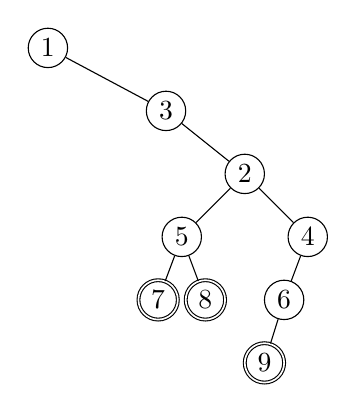
\begin{tikzpicture}[level distance=0.8cm,
        level 1/.style={sibling distance=3cm},
        level 2/.style={sibling distance=2cm},
        level 3/.style={sibling distance=1.6cm},
        level 4/.style={sibling distance=0.6cm},
        level 5/.style={sibling distance=0.5cm},
        every node/.style={draw,circle,inner sep=0pt,minimum size=5mm}]
        \node {1}
        child[missing]
        child {
            node {3}
            child[missing]
            child {      
                node {2}
                child {
                    node {5}
                    child {
                        node[circle,double]{7}
                    }
                    child {
                        node[circle,double]{8}
                    }
                }         
                child {
                    node {4}
                    child {
                        node {6}
                        child {
                            node[circle,double]{9}
                        }
                        child[missing]
                    }
                    child[missing]
                }
            }
        }
        ;
    \end{tikzpicture}
\end{center}